\chapter{Martensitzerfall}

\section{Durchführung (TJ)}

Für die weitere Wärmebehandlung soll in einem dritten Schritt der vorher gebildete Martensit partiell zum Zerfall gebracht werden. Ein Anteil der $\alpha'$-Nadeln wandelt sich in $\alpha$- und $\beta$-Phase um. Damit soll sich eine weitere Verfeinerung der Struktur ergeben, die zu einer Festigkeitssteigerung führt. Diese partielle Dekomposition soll gleichzeitig zu einer Duktilitätssteigerung sorgen \cite{Lutjering.2007}.

Dazu wurde die Probe aus Abbildung \ref{fig:abbildung-18} (983$^\circ$C/1h/AC + 950$^\circ$C/16min/WQ), die die ausgeprägtesten Martensitstrukturen aufwies, für die weiteren Schritte ausgewählt. 
Dafür wurden vier Proben für den dritten Wärmebehandlungsschritt festgelegt. Zwei Proben wurden bei 580$^\circ$C und unterschiedlichen Haltezeiten (8 und 16 min) wärmebehandelt. Die zwei verbliebenen wurden den gleichen Haltezeiten ausgesetzt, nur bei höher Temperatur (610$^\circ$C).
Die Temperatur von 580$^\circ$C wurde aus der Ausgangsstudie übernommen. Aufgrund der Erfahrungen des zweiten Wärmebehandlungschritts (Martensitbildung) wurde zusätzlich eine höhere Temperatur (610$^\circ$C) gewählt.
Es wurden längere Haltezeiten im Vergleich zur Ausgangsstudie genommen, da die verwendete Probendicke größer ist.

\section{Ergebnisse (PH)}

Die Analyse unter dem Lichtmikroskop ergab keine sichtbare Veränderung der Mikrostruktur zur vorherigen Probenreihe. Die Ergebnisse der weiteren Auswertung unter dem REM sind in den Abbildungen \ref{fig:abbildung-22} -- \ref{fig:abbildung-25} zusammengefasst.

\begin{figure}
	\centering
	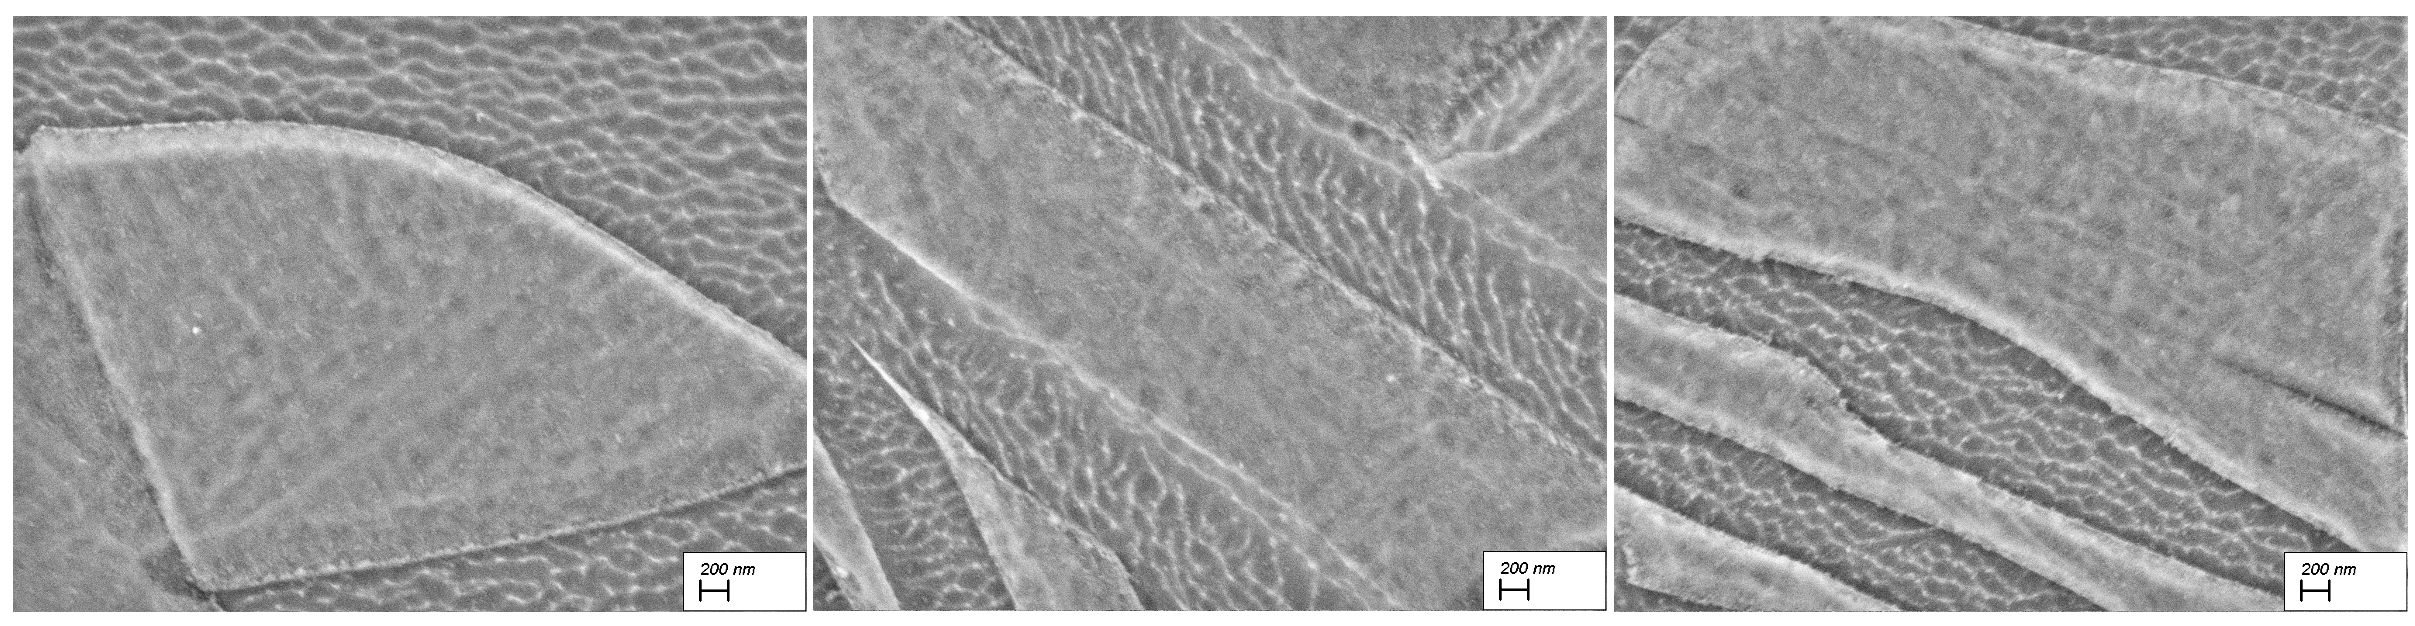
\includegraphics[width=1.0\linewidth]{./Bilder/Abbildung 22.png}
	\caption[Abbildung 22]{983$^\circ$C/1h/AC + 950$^\circ$C/16min/WQ + 580$^\circ$C/8min/AC, REM}
	\label{fig:abbildung-22}
\end{figure}

\begin{figure}
	\centering
	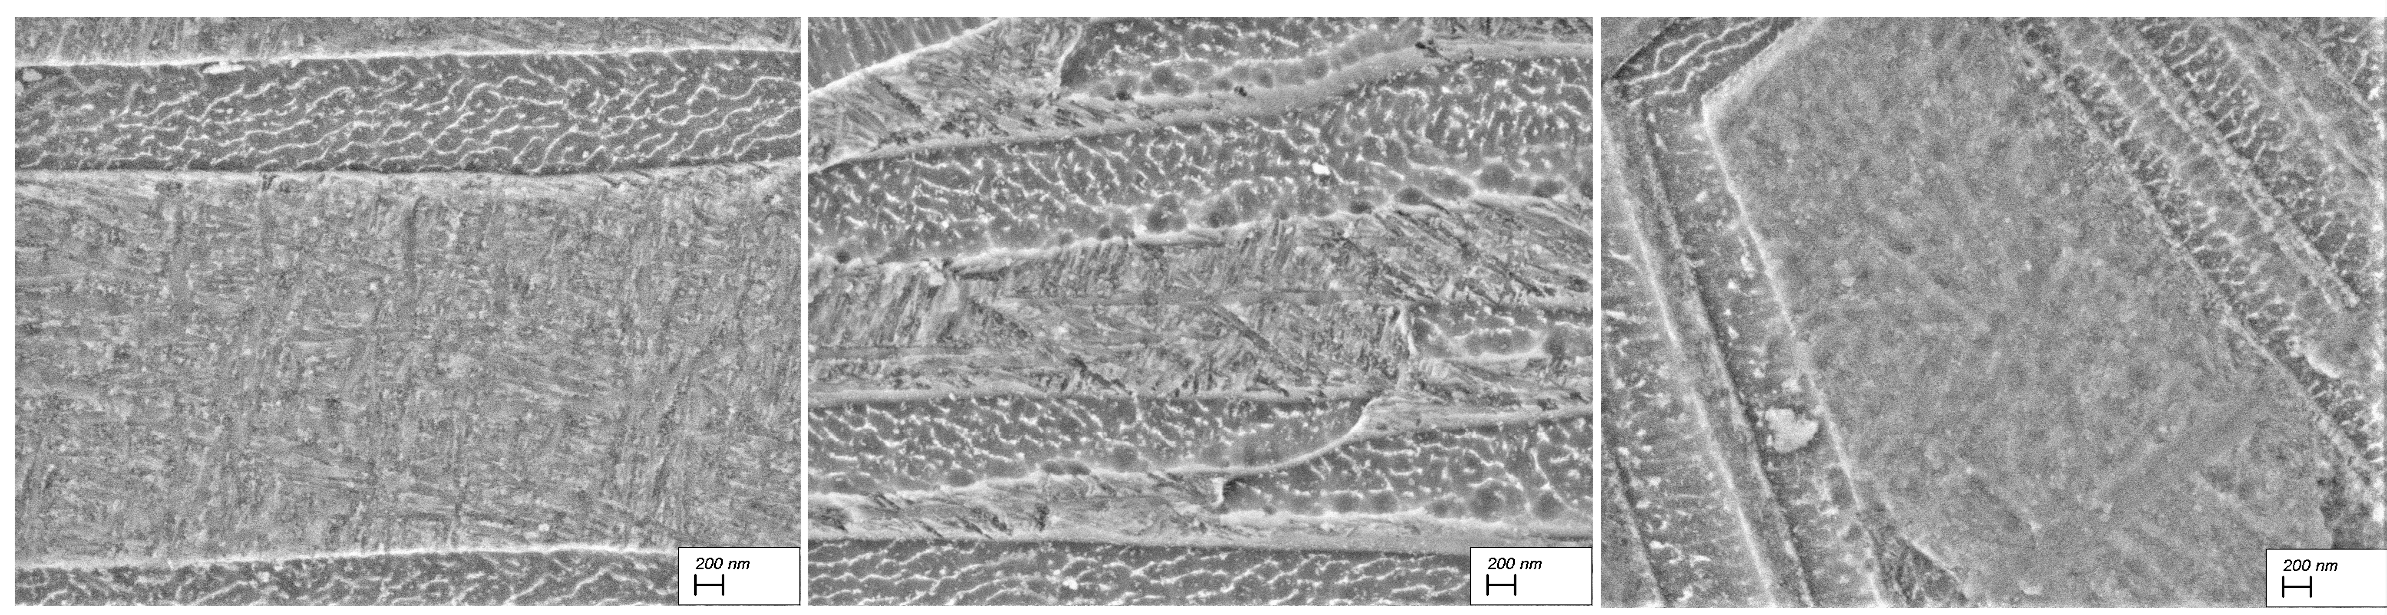
\includegraphics[width=1.0\linewidth]{./Bilder/Abbildung 23.png}
	\caption[Abbildung 23]{983$^\circ$C/1h/AC + 950$^\circ$C/16min/WQ + 580$^\circ$C/16min/AC, REM}
	\label{fig:abbildung-23}
\end{figure}

\begin{figure}
	\centering
	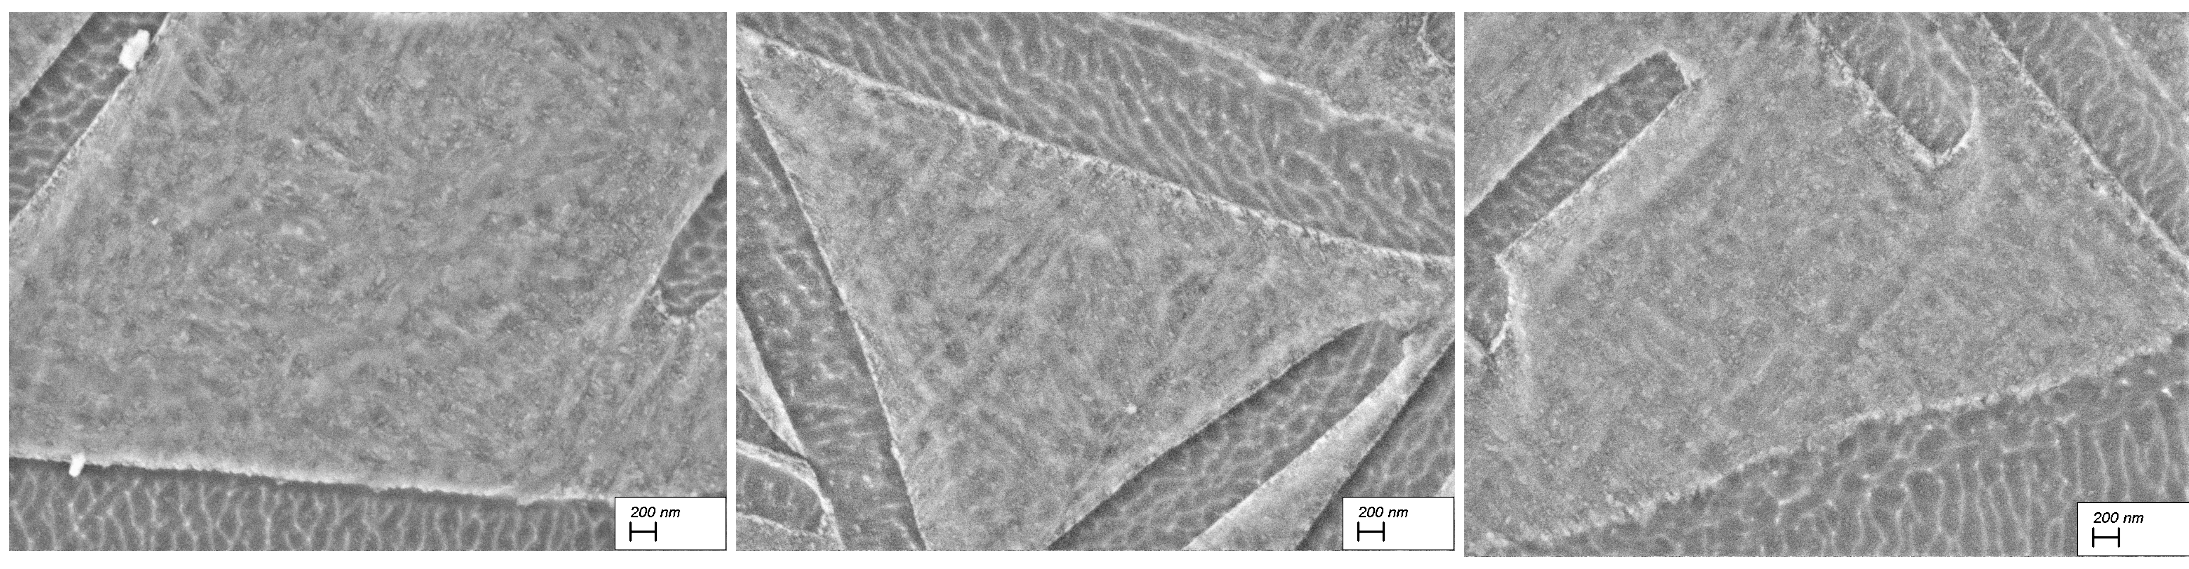
\includegraphics[width=1.0\linewidth]{./Bilder/Abbildung 24.png}
	\caption[Abbildung 24]{983$^\circ$C/1h/AC + 950$^\circ$C/16min/WQ + 610$^\circ$C/8min/AC, REM}
	\label{fig:abbildung-24}
\end{figure}

\begin{figure}
	\centering
	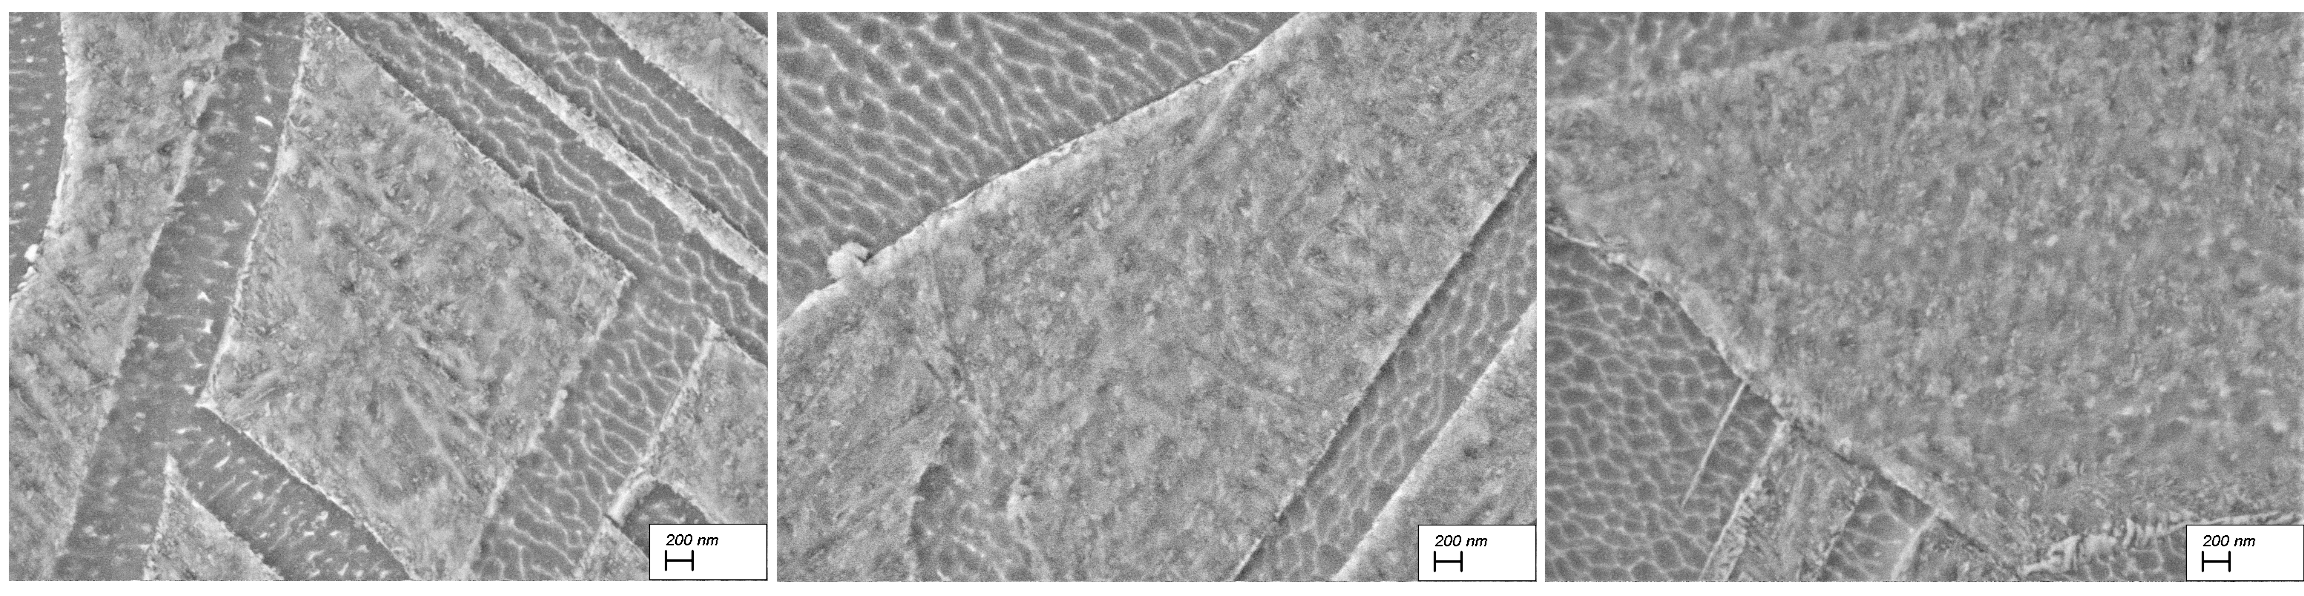
\includegraphics[width=1.0\linewidth]{./Bilder/Abbildung 25.png}
	\caption[Abbildung 25]{983$^\circ$C/1h/AC + 950$^\circ$C/16min/WQ + 610$^\circ$C/16min/AC, REM}
	\label{fig:abbildung-25}
\end{figure}

In den Abbildungen \ref{fig:abbildung-22} -- \ref{fig:abbildung-25} ist zu sehen, dass die Martensitstrukturen in der $\beta$-Phase zum größten Teil zerfallen sind. Es sind nur an vereinzelten Stellen der Proben noch ansatzweise Rückstände dieser Strukturen zu erkennen.

Die Härteprüfung zeigte im Gegensatz zur vorherigen Probenreihe eine signifikante Härtesteigerung. Die Ergebnisse sind in Tabelle \ref{Tabelle 8} zusammengefasst.

\begin{table}
	\centering
	\begin{tabular}{|c|c|}
		\hline 
		Probe & Härte in HV \\ 
		\hline 
		983$^\circ$C/1h/AC + 950$^\circ$C/16min/WQ + 580$^\circ$C/8min/AC & 393 \\ 
		\hline 
		983$^\circ$C/1h/AC + 950$^\circ$C/16min/WQ + 580$^\circ$C/16min/AC & 392 \\ 
		\hline 
		983$^\circ$C/1h/AC + 950$^\circ$C/16min/WQ + 610$^\circ$C/8min/AC & 399 \\ 
		\hline 
		983$^\circ$C/1h/AC + 950$^\circ$C/16min/WQ + 610$^\circ$C/16min/AC & 392 \\ 
		\hline 
	\end{tabular} 
	\caption{Ergebnisse der Härteprüfung nach dem Martensitzerfall}
	\label{Tabelle 8}
\end{table}

\section{Diskussion der Ergebnisse (TJ)}

Die Erbebnisse haben gezeigt, dass die Martensitstrukturen nur noch an vereinzelten Stellen auftreten. Die Umwandlung ist jedoch nicht soweit fortgeschritten, dass einzelne $\alpha$- und $\beta$-Körner sichtbar sind.
Dadurch hat der Martensitzerfall nur partiell stattgefunden.\\
Es ist deshalb ein signifikanter Härteanstieg vom zweiten auf den dritten Schritt zu erkennen. 



